\documentclass[UTF8]{csoarticle}

\begin{document}

\titleCHN{基于层次注意力机制的远程监督关系抽取算法研究}
\titleENG{Distantly Supervised Relation Extraction with Layered Attention Mechanism}
\authorCHN{陈元昆\affil{},刘建毅\affil{}}
\authorENG{CHEN Yuankun\affil{}, LIU Jianyi\affil{}}
\affiliationCHN{
    \affil{} 北京邮电大学网络空间安全学院,北京 100876
}
\affiliationENG{
    \affil{} School of Cyberspace Security, Beijing University of Posts and Telecommunications
    , Beijing 100876 \\
}
\abstractCHN{
远程监督机制由于其使用机器自动标注数据,能减少大量标注人力的优点,
逐渐成为了知识图谱构建中关系抽取任务的主要手段。目前,如何能够较好的提取句子特征,
为句子分类(关系抽取)提供良好的分类依据,成为了远程监督领域的一个研究课题。
为了解决这个问题,本文采用了称为层次注意力机制的网络结构,
该网络结构将注意力机制组织为层次结构,以更好地应对数据噪声,捕获句子的特征。
本文使用注意力机制作为句子和句袋这两个层次特征的主要的编码器,
构建了一个抗噪能力较强的远程监督机制的关系抽取器。
实验表明,该模型在捕获句子特征、增强泛化能力方面超过了现有模型。
}
\abstractENG{Distant Supervision has gradually become a main method in Knowladge
graph construction due to it reduced the manpower of annotating data because 
it uses machines to automatically annotate data. At present, 
how to better extract sentence features and provide good 
classification basis for sentence classification (relation extraction) 
has become a research topic in the field of distant supervision. 

    To solve this problem, this paper uses a network structure
called the hierarchical attention mechanism, 
which organizes the attention mechanism into a hierarchical structure 
to better deal with data noise and capture the characteristics 
of sentences. 

    In this paper, attention mechanism is used as the main encoder of 
two levels of features: sentence levle and sentence bag level, 
and a relational extractor with strong anti-noise ability and 
distant supervision mechanism is constructed. 
Experiments show that the model outperforms existing models in
 capturing sentence features and enhancing generalization capabilities.}  
\keywordCHN{深度学习\ 自然语言处理 \ 知识图谱 \ 关系抽取\ 注意力机制\ 远程监督}
\keywordENG{Deep learning, Natural Language Processing, Knowladge Graph, Relation Extraction. Attention Mechanism, Distant Supervision}
\cateidCHN{TP181}

\authorIntroduction{陈元昆(1995-),男,硕士研究生在读,主要研究方向:知识图谱,自然语言处理。通信作者:刘建毅(1980-),男,副教授,主要研究方向:数字内容安全,智能信息处理,数据挖掘。E-mail:liujy@bupt.edu.cn}

\maketitle


%----------------------------------------------------------
% 2. 正文内容
%----------------------------------------------------------

\section{引言}
随着知识图谱技术在金融,风控,情报,个性化推荐等领域中发挥越来越重要的作用。
快速地自动化地构建知识图谱,尤其是其子任务实体识别和关系抽取,
成为了自然语言处理领域的重要研究课题。
远程监督机制\cite{bib1},启发式地将知识库中的三元组与分结构化文本对齐,
自动化地标注大量训练数据,不用耗费大量人力物力去手动标注,
为构建大规模标注语料库找到了更快的方法,逐渐成为了现在关系抽取领域的一个重要工具。
远程监督机制基于一个最基本的假设:
如果两个实体\textbf{$e_1$}和\textbf{$e_2$}之间存在关系\textbf{r},
那么语料库中所有包含这两个实体的句子,都认为可以表述关系\textbf{r},
也会被标注为关系\textbf{r}的训练实例。
例如,在知识库中给定实体对\textbf{姚明},\textbf{上海},
以及他们之间的关系 \textit{place\_of\_birth},
可以将语料库中所有同时包含实体\textbf{姚明}, \textbf{上海}的句子标注,
认为它们表达了关系\textit{place\_of\_birth}。

远程监督尽管明显降低了用于标注的海量人力和时间,但由于其依赖于一个过于绝对的假设,所以总是会构建出一个充满了错误标注噪声的训练数据。
在现实世界中,往往不是每一个句子都会表述想要的关系。例如,"姚明,生于中国上海市,祖籍江苏省苏州市吴江区震泽镇,著名篮球运动员",表述了\textit{place\_of\_birth}关系,
而句子“2009年,姚明收购上海男篮,成为上海大鲨鱼篮球俱乐部老板。”并不能体现这个关系。
在真实世界中,远程监督标注的数据总是有着大量类似的噪声数据,有时受限于语料库的质量,关于一对实体的标注数据甚至可能一个正确的实例都没有,这也造成了基于远程监督训练的深度学习模型性能普遍一般。
在单个句子分类能力已经达到了较好水平的情况下,在充满了大量噪声的远程监督数据上,如何训练一个能克服噪声性能良好的分类器,成为了当下研究者关注的重点


为了缓解应对远程监督带来的大量噪声问题,Ridel\cite{bib2} 等人提出来了多实例学习方法。
Ridel将远程监督的假设放宽松,首先将标注为一对实体某个关系的所有句子实例称为一个句袋(sentence bag),
Ridel等人认为一个句袋中至少可以有一个句子实例表述了标注的关系,这也称为“至少一个”假设(at least one assumption)。在学习中我们可以只学习一个句袋中最有可能的句子实例,大大降低了噪声数据带来的影响,提升了提取器的性能。
使用了“至少一个”假设学习策略的提取器,最大的瓶颈是在句子特征提取上。

句子特征提取,是关系抽取的基础,一个良好的句子特征表示,可以为后续的关系分类奠定基础。
对于长度可变的自然语言文本,如何提取长句子中的隐含依赖关系,是自然语言理解中的重要难题。
早期的学者们常常依赖于外部的自然语言处理工具对于句子及进行词性标注、依存分析等作为句子的特征标注。
这类句子特征生成的最大问题是特征的准确度依赖于这些工具,如果这些工具的准确率不高,也会对后续的分类准确度有着一定的影响。
其次,当句子过长,这类标注工具的准确率会急剧下降。

鉴于深度学习方法在图像领域取得了巨大的成功,自然语言领域也引入了这一强有力的工具,用来自动化地提取自然文本的语义特征。
卷积神经网络(PCNNs)\cite{bib3},长短时记忆网络(LongShort Term Memory Network)\cite{bib4} 等都在关系抽取领域的句子特征提取上取得了成功。
然而,CNN与LSTM在提取长序列的语义特征上,依然有其天然的不足。CNN由于卷积核尺寸的限制,无法很好的捕获一个长距离的依赖关系。
而LSTM虽然克服了RNN在长距离依赖上的梯度消失问题,却依然不能够很好的理解距离过于远的依赖关系。

为了能够有效地降低训练数据中的噪声,除了上文中所提到的“至少一个”策略,软注意力机制也被广泛使用。
软注意力机制在句袋内部,通过计算每一个句子与最终结果的相似度,实现了注意力权重的再分配,有效地利用了句袋内的噪声与非噪声信息。

为了解决远程监督中句子特征提取和降噪问题,本文提出了层次的注意力机制,基于自注意力机制,能够快速高效的在句子层面提取特征,并且在句袋层面降低噪声。
本文使用了一个基于自注意力机制的句子编码器,能够更好的捕获句子中的任意两个单词之间的长期依赖关系,在不需要自然语言特征标注工具的情况下,得到了一个有更好表示效果的句子特征。
其次,在句袋层面,同样采用了一个基于注意力机制的句袋编码器,能够更好的在充满噪声数据的句袋中捕获有效信息。在提升
实验结果表明本文提出的句子编码器能够比现有模型模型取得更好的句子编码效果。

\section{相关工作}
为了解决在有监督的关系抽取研究中标注数据较少的问题,Minz\cite{bib1}等人提出了一种称为远程监督(Distant Supervision)的标注方法。
该方法利用已有的知识库,启发式地将知识库中现存的三元组与语料对齐,从而自动化地获得大量的的标注数据。
然而远程监督假设过于绝对,其认为只要一个句子中有两个在知识库中的实体,并且这两个实体在知识库中存在关系\textit{r},就认为这个句子表述了关系\textbf{r},并将其标注为\textbf{r}。
这个绝对的假设,也为远程监督的标注的数据集带来了海量的噪声。

为了解决远程监督带来的噪声问题,多实例学习首先被Ridel\cite{bib2}等人提出,该方法采用了一个更为宽松的假设,假设含有同一对实体且标注为关系\textit{r}的所有句子中,至少有一对确实表述了关系\textit{r}。
以上的学习方法多依赖于手工特征或者使用外部标注工具标注的特征作为句子特征,严重依赖于标注的准确性,也会导致误差传播问题。

为了解决在关系抽取时句子特征的提取问题,深度学习随着在其他领域的大获成功,也逐渐被引入了关系抽取领域。Zeng\cite{bib3} 等人首次提出了使用PCNNs作为特征提取器。
PCNNs网络将句子从实体对断开成三段,在三段上分别使用最大池化,一定程度上提取了句子的结构信息。
Zhou\cite{bib4}等人提出BILSTM-Attention模型使用BiLSTM模型和句子间的注意力机制,更好捕获了句子中的长期依赖关系。

2017年来,注意力机制进入了人们的视线,首先是Lin \cite{bib5}等人将软注意力机制应用在远程监督的句袋间降噪上,使用了句袋间的软注意力机制,将句袋间所有句子的加权和作为句袋特征,达到了良好的降噪效果。
Vaswani\cite{bib6}等人提出了自注意力机制,该机制能够更好地捕获长距离序列中各单词之间的依赖关系,同时通过并行化的方法,大大减小了运算时间,提升了效率。
以自注意力机制为核心的Transformer网络和BERT语言模型也在机器翻译,对话以及各种下游任务上取得了最好的效果。
受到自注意力机制的启发,本文提出了使用注意力模型为核心的句子编码器。在句子特征选择上,我们使用自注意力机制结合句间软注意力机制,更好的捕获了句子特征,对于下游的关系抽取效果也有了一定的提升。
\section{算法模型}
\begin{figure}[ht]
    \centering
    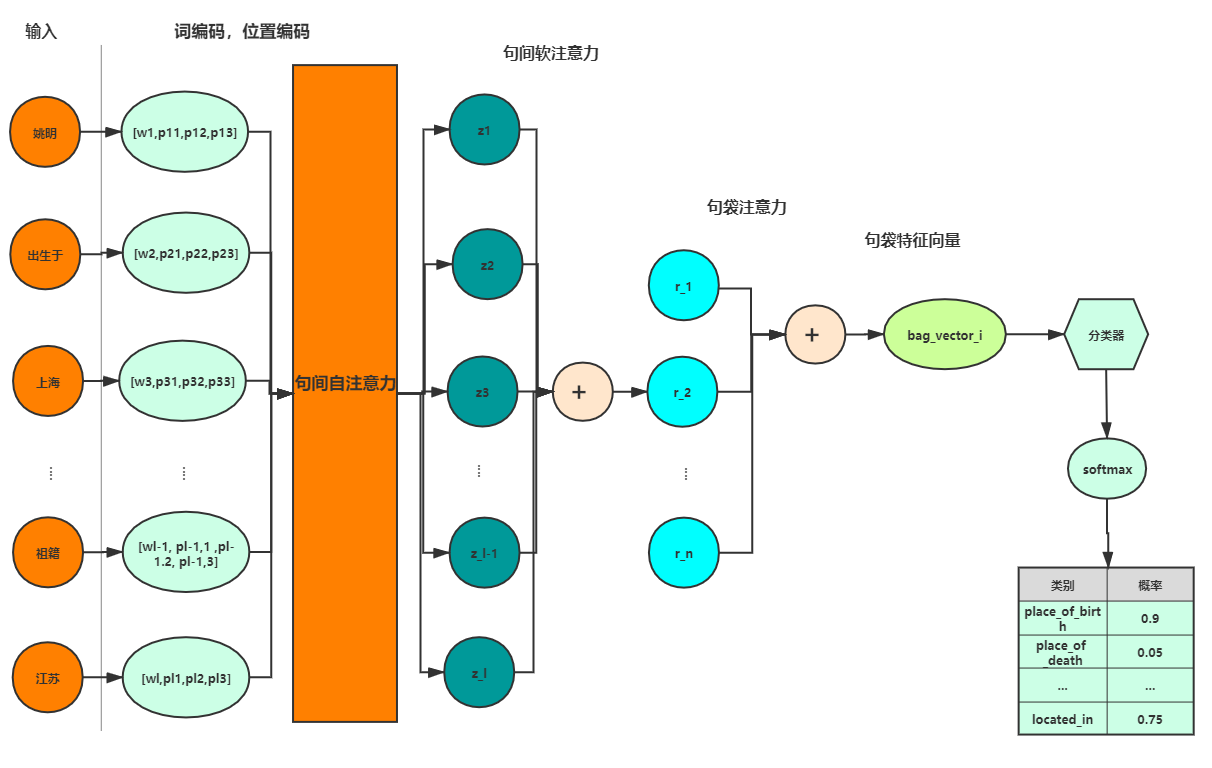
\includegraphics[width=1 \textwidth]{structure.png}
    \caption{模型结构图}
    \label{fig:fig1}
    \end{figure}
本章主要介绍层次注意力机制的主要结构。
如图所示,模型主要由两个模块组成:句子特征提取器和句袋特征提取器。第一部分主要通过自注意力机制计算数据中每一个句子的特征,可以将含有实体对的自然文本转变成一个定长为$d_{hidden}$的实值向量。
其次是一个句袋特征提取器,同样使用自注意力机制,在句袋内部通过注意力机制的权重,对所有句子的特征向量进行重新分配。达到了较好的降噪效果。
\subsection{句子表示学习}
\subsubsection{词编码}
词编码主要任务是高维稀疏的独热词编码转化为稠密低维的向量表示,方便计算机处理和运算。一个好的词向量,不仅能把单词降维,还可以提供额外的单词语义信息。
目前公认使用预训练好的词向量能够对下游任务有较好的提升,当前最主流的词编码是Thmos\cite{bib7}等人提出的Word2Vec词向量。Word2Vec使用cbow和skipgram方法,分别在维基百科上进行训练。
\subsubsection{位置编码}
在本文的算法网络结构中,由于attention模型对于序列中单词的顺序不敏感,需要在单词编码中加入位置信息。此外,由于关系抽取情景下,一个句子中最主要的信息是两个实体,所以我们此外还要加入每个单词到句子中两个实体的相对位置信息(实验证明有没有用??)。
对于一个输入的句子$S_i={w_1, w_2, ..., w_l}$,其中$w_i$表示句中的一个单词,l表示句子的长度,我们将每一个单词$w_i$最终映射为维度为$ d=d_{word} + 2*d_{relative\_position} + d_{absolute\_position}$

\subsubsection{句子特征提取}

如上文所述,本文使用自注意力机制作为句子级别的特征提取器。
对于一个句子S,其维度为$d_s\in R^{l\times w}$
首先将句子经过h个多头注意力,每一个注意力头$head_j$通过不同的三个矩阵将同一个句子映射成3个$d_{f}$维向量组成的向量组$\{\boldsymbol q_j=W_j^{q}S, \boldsymbol k_j=W_j^{k}S, \boldsymbol v_j=W_j^{v}S\}$
每一个向量组经过一个Scale Product attention头进行如下计算

\[ att\_vector_{j} = softmax(\frac{q_{j} k_{j}^{T} }{\sqrt{dim_k}})v_{j}\]

其中$att\_vector_j$的维度与$q, k, v$相同,
然后将所有$att\_vector$串联成
\[attn = Cat\{att\_vector_1,att\_vector_2,...,att\_vector_h\}\]
其中 $attn$ 维度为$d_{attn} \in R^{l\times w}$
最后通过一个矩阵将$attn$映射为$Output$, 维度$d_{O} \in R^{l\times d_{hidden}}$

对于一个批次的n个句子组成的矩阵$Input={S\_1, S\_2,...,S\_n}$, 维度$d_{I} \in R^{n\times l\times w}$
通过句子特征提取器,得到$Output={b\_1, b\_2,...,b\_n}$,其维度$d_{O} \in R^{n\times l\times  d_{hidden}}$

\subsubsection{句子级别软注意力机制}
自注意力机制能够将句子各单词根据彼此之间的依赖关系分配权重,
并且根据分配到的权重加权得到每一个单词的新的向量表示。
现有使用自注意力机制进行句子特征提取的方式,往往在句子间向量重组后使用最大池化(Max Pooling)或者平均池化(Mean Pooling)。这类对于蒸馏句子特征的方式,总是认为句子中的各个单词只有一个对特征有贡献,或者所有都有同样贡献,这个观点过于直接,并且违背直觉。
一个句子能否表示一个关系,其中每一个单词起到的贡献度是不同的。
比如句子“姚明(Yao Ming),男,汉族,无党派人士,1980年9月12日出生于上海市徐汇区,祖籍江苏省苏州市吴江区震泽镇。”,
对于关系\textit{place\_of\_birth}贡献最大的无疑是短语“出生于”,但是其中的“1980年9月12日”,“祖籍江苏省苏州市吴江区震泽镇”,两部分,也是在介绍人物出生地的时候常常会一起出现的语法结构。
由此可见在确定一个句子的关系时,句中的很多成分都能起到一定的促进作用。
Zhou\cite{bib4}等人在BiLstm处理后的句子特征序列上使用了软注意力机制求得各单词向量的加权和。
受到Zhou等人的启发,本文同样在自注意力编码得到的句子序列特征上同样使用软注意力机制,将句子序列的各部分进行加权求和。获取一个更加能够包含句子各部分信息的句子向量。
实验结果证明,本文的改进对句子特征提取起到了促进作用。

对于每一个输出的句子向量$ b\_i = {z\_1, z\_2,...,z\_l} \in R^{l \times d_{hidden}} $
将其通过如下运算,得到每一个单词在序列中的权重$\alpha$,并且加权求和后得到句子的特征向量r。
\[ M= \tanh(b\_i) \]
\[ \alpha = softmax(w^T M) \]
\[ r\_i = b_i \alpha^T \]

\subsection{句袋特征提取}
句袋特征提取将一个句袋中的所有句子整合成一个句袋向量$bag\_vector$。

一个句袋包含了语料库中所有提及实体对$(e1, e2)$的句子。
在句袋中,每一个句子都是由句子编码器中输出的句子特征向量 $r \in R^{d_{hidden}}$所表示。
一个句袋可以表示为矩阵$B \in R^{n \times d_{hidden}}$
对于每一个句袋,同样使用一个选择性注意力机制,将一个句袋内的句子特征进行重新分配。
我们认为这样可以将句袋中的句子根据与关系的相近程度分配权重。
对于一个输入的句袋$B = \{b_b1, b_2,...,b_t\}$,其中t表示一个句袋中的句子个数。
根据一个句子特征向量相对于其真实关系向量$r_i$的相似度,提取句袋特征向量$b_i$。
\[attention\_score_i =  b_i\cdot W_r \cdot r_i\]

其中$W_r$的维度$d_{W_r} = R^{d_{hidden}}$。

对于一个句袋,其中每一个句子$a_i$都可以计算得到一个注意力得分$attention\_score_i$,
将注意力得分归一化,得到每一个句子对应的注意力权重。
\[\alpha = softmax({a_1,a_2,...,a_t})\]

最后求各句子向量的加权和,得到一个句袋的特征表示向量
\[bag\_vector = sum(\alpha  B)\]

上文中$attention\_score_i$, $bag\_vector$的维度分别为$d_T$,$d_{hidden}$。

\subsection{训练}
在深度学习领域,训练的目的是通过梯度下降和反向传播算法,在迭代中不断减小算法输出与真实情况的差距。
本文选择交叉熵函数用于衡量网络输出与真实情况的差距的目标函数,不断更新网络的参数。
在本文的网络中交叉熵公式如下:
\[ CE =-\sum _{i}y_i \log q_i\]

其中$y$是一个句袋独热形式的真实标签,$q$是网络输出的一个句袋在所有标签上的得分。
\section{实验与评估}
本章将本文提出的模型与现有的模型进行对比实验。
实验在处理器 Intel Core i9-9820X 3.30GHz 显卡 RTX 2080TI 11G, 内存 32G 的计算机上进行训练的。

\subsection{数据集与评价标准}
本文使用了Ridel\cite{bib2}等人提出的远程监督标准数据集NYT-10。该数据集将Freebase知识库与纽约时报的语料对齐,现在已经成为了大量方法的评价数据集
NYT10数据集中一共有52种关系外加一个NA关系。
其中训练集包含522,611个句子, 281,270对实体,测试集包含172,448个句子和96,678个实体对。
本文使用了留出法作为模型验证方法,只在训练集上训练模型,只在测试集上测试模型。
本文还使用在不同召回率下的准确率作为评价指标。

\subsection{训练设置}
为了方便比较,与前人工作\cite{bib3, bib4}相同,本本文设置词嵌入向量维度为50,每一个位置嵌入向量维度为5。
选择230为句子向量的维度,同样也将句袋特征的维度设置为230。
在自注意力的句子编码器内部,本文将多头注意力的头个数$n\_heads$设置为5,以便将65维的单词向量在多头注意力中平均地映射。
此外我们将注意力模块的个数$n\_blocks$设置为1。

本文使用了Adma优化器来通过反向传播更新模型参数,初始学习率设置为0.001。此外,在输出层使用Dropout用以防止模型过拟合。
\subsection{结果比较}
将本文的模型与Sun\cite{bib12}提出的MSnet模型进行对比。
对每个模型训练20轮,挑选效果最好结果的进行对比,本文主要选取P@0.1, P@0.2, P@0.3, Max F1 这四个指标,
主要衡量了分类器在不同召回要求的情况下分别对应的分类准确性,以及分类器整体的准确率召回率的均衡性。

\begin{figure}[ht]
\centering
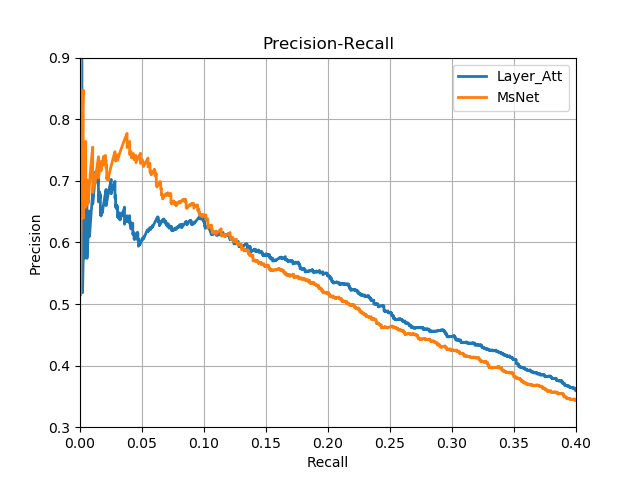
\includegraphics[width=0.9\textwidth]{pr_curve.png} 
\caption{Precision-Recall曲线}
\label{fig1}
\end{figure}


\begin{table}
\begin{center}

\begin{tabular}{l||c|c|c|r|}
Model & P@0.1 & P@0.2 & P@0.3 & Max F1\\
\hline
Layer\_Att& 0.6379          & \textbf{0.5512}& \textbf{0.4572}& \textbf{0.3844} \\
MSnet     & \textbf{0.6468} & 0.5147         & 0.4328          & 0.3691 \\
\end{tabular}
\end{center}

\caption{指标对比}
\label{tab1}
\end{table}


从图\ref {fig1} 和表\ref {tab1}中可以看出,相比于Sun\cite{bib12}的模型,本文的模型虽然在召回率为0.1时候对应的准确率上略逊一筹,
但是在召回率大于0.1的时候,模型的准确率始终优于Sun的模型。此外,本文的模型在整体的AUC指标,MaxF1指标上都要超出一些,
这是因为加入句子级别软注意力机制后,对句子的特征提取不再局限于某些单词,而能够考虑到更多潜在的语义特征。
尤其从PR的曲线走势上,可以认为,本文提出的基于层次注意力的关系抽取模型是更加有泛化能力的、更优秀的模型。
\subsection{模型效率分析}
自注意力机制相比与传统的串行的注意力机制,能够快速并行,在时间效率上远远超过了传统的序列编码模型,如RNN(LSTM, GRU)等人提出来了多实例学习方法。
在训练集上分别训练了本文提出的多头注意力编码器,BiLstm和BiGRU,每个模型训练五轮,取一个轮次的平均计算时间进行对比。结果如下:

\begin{table}[!htbp]
\begin{center}
    \begin{tabular}{|l|c|r|}
    模型 & 运行速度(耗费时间(s)/每轮次(epoch)) & 最好效果(AUC)\\
    \hline  
    Layer\_Att &309 & \textbf{0.2197}  \\
    % MSnet &\textbf{205}& 0.2572 \\
    BiLstm & 334& 0.1440\\
    BiGRU & 323& 0.1183\\
    \end{tabular}
    \caption{运行效率对比}
\end{center}

\end{table}

从上表可以看出,同样的参数情况下,本文使用自注意力机制的关系抽取器在运行速度上快于BiLstm和GRU。
此外,在同样的训练轮数和后本文的模型在测试集上达到了更好的的效果,说明该模型同样的优化函数下收敛的更快。

\section{结论}
关系抽取是自然语言处理、知识图谱领域的重要子任务。研究如何快速高效的从语料库中识别实体之间的关系,为构建知识图谱提供了良好的基础,
也是知识图谱在金融、征信、风控、医疗等领域发挥重要作用的第一步。
本文将自注意力机制结合软注意力机制,在句子特征提取方面对现有模型进行了改进。实验结果表明,本文提出的算法模型在一些指标上赶上和超过了现有模型。
注意力机制是近年来自然语言处理领域的一个重要的工具,在文中选用的软注意力是利用一个映射矩阵自动将句子向量映射成权重信息,此外没有考虑到更多的外界信息。
在关系抽取领域,实体和关系级别的信息都对于关系抽取有着重要的影响,这也是=下一步构建一个更好的句子特征选择算法索要考虑到的
在研究中发现,由于知识库的局限性,远程监督标注数据大部分标签是无效信息NA,在训练中并没有充分利用这部分信息,
这也导致模型的学习效率和最终性能与其他领域类似任务相比有很大差距。这一点也是进一步的研究重点。
\section*{致谢}
感谢我的指导老师,张茹,刘建毅老师,在论文撰写和实验进行期间给我提出的纲领性意见,高屋建瓴,让我在研究领域有了不一样的思路。

感谢论文撰写期间各位对我提供帮助的同学和朋友。

感谢我所在的灾备技术国家工程实验室,为我提供实验所需的各种软硬设施。

\begin{thebibliography}{15}
    \bibitem{bib1} Mike Mintz, Stevens Bills, Rion Snow, et al. Distant supervision for relation extraction without labeled data, Proceedings of the 47th Annual Meeting of the ACL and the 4th IJCNLP of the AFNLP, 2009.
    \bibitem{bib2} Riedel Sebastian, Yao Limin, McCallum Andrew , Modeling relations and their mentions without labeled text, Proc. Joint Eur. Conf. Mach. Learn. Knowl. Discovery Databases, Berlin, Germany: Springer, 2010.
    \bibitem{bib3} Zeng Daojian, Liu Kang, Chen Yubo, et al., Distant Supervision for Relation Extraction via Piecewise Convolutional Neural Networks, Proceedings of the 2015 Conference on Empirical Methods in Natural Language Processing, 2015.
    \bibitem{bib4} Zhou Peng, Shi Wei, Tian Jun, et al.,  Attention-Based Bidirectional Long Short-Term Memory Networks for Relation Classsification, Proceedings of the 54th Annual Meeting of the Association for Computational Linguistics, 2016.
    \bibitem{bib5} Lin Yankai, Shen Shiqi, Liu Zhiyuan, et al., Neural Relation Extraction with Selective Attention over Instances, Proceedings of the 54th Annual Meeting of the Association for Computational Linguistics, 2016.
    \bibitem{bib6} Vaswani,Ashish,Shazeer Noam,Parmar Niki,et al., Attention Is AL You Need,31st Conference on Neural Information Processing Systems (NIPS 2017), Long Beach, CA, USA, 2017.
    \bibitem{bib7} Thome Mikolov, Sutskever Ilya , Chen K, et al., Distributed representations of words and phrases and their compositionality, Neural information processing systems, 2013.
    \bibitem{bib8} Ji Guoliang, Liu Kang, He Shizhu, et al., Distant Supervision for Relation Extraction with Sentence-Level Attention and Entity Descriptions, Proceedings of the Thirty-First AAAI Conference on Artificial Intelligence, 2017.
    \bibitem{bib9} Yuan Yujin, Liu Liyuan, Tang Siliang, et al., Cross-Relation Cross-Bag Attention for Distantly-Supervised Relation Extraction,Thirty-Third AAAI Conference on Artificial Intelligence (AAAI-19), 2019.
    \bibitem{bib10} Cai Rui, Zhang Xiaodong, Wang Houfeng, Bidirectional Recurrent Convolutional NeuralNetwork for Relation Classsification, Proceedings of the 54th Annual Meeting of the Association for Computational Linguistics, 2016.
    \bibitem{bib11} Zeng Daojian, Liu Kang, Lai Siwei,et al., Relation Classification via Convolutional Deep Neural Network,Proceedings of COLING 2014, the 25th International Conference on Computational Linguistics, 2014.
    \bibitem{bib12} Sun Tingting, Zhang Chunhong, Ji Yang, et al., "MSnet: Multi-Head Self-Attention Network for Distantly Supervised Relation Extraction", Access IEEE, vol. 7, pp. 54472 - 54482, 2019.
    
\end{thebibliography}

\end{document}
